This chapter shows the experimental results of our proposed HALNS algorithm in comparison with the defined baseline methods. It also analyzes the adaptive weight adjustment and details the parameter selection process.

\section{Experimental results}

    Here, we compare our proposed HALNS algorithm described in section \ref{sec:halns} with the three baseline methods detailed in section \ref{sec:baseline}. The experiments were conducted on the benchmark datasets, which are illustrated in section \ref{sec:dataset}. Each dataset consists of 10 instances with the same number of requests and drivers. Each experiment on each instance was executed 10 times and the results were averaged. All experiments were conducted on a machine with a 2,6 GHz 6-Core Intel Core i7 processor and 16 GB of RAM, and the maximum running time was restricted to 10 minutes. The ORTools baseline method is unable to reasonably solve instances containing more than 20 requests. Therefore, the ORTools method was evaluated only on the smallest instance containing 20 requests.
    
    For comparison of the algorithms, we use the metrics M1 to M5 introduced in section \ref{sec:metrics} rather than the objective value. The reason is that these metrics provide much deeper insight into the quality of the produced solutions. Table \ref{tab:delay} contains the experimental results in the context of the M1 metric, which indicates the average (and maximum) delay per single request at its drop-off location. Similarly, Table \ref{tab:distance} highlights the M2 metric results, which indicates the average (and maximum) distance driven by each driver. In both tables, the minimum values are in bold to feature the best algorithm per each dataset. All five metrics M1 to M5 are then visualized in figure \ref{fig:metrics-graphs}. For each metric, we show the average value per each dataset and method along with the standard deviation. In the mentioned tables and figures, \emph{IH} stands for insertion heuristics baseline method, and \emph{IH \& ORTools} refers to the combination of insertion heuristics and ORTools, which is one of the baseline methods described in section \ref{sec:baseline}.

    The results in tables \ref{tab:delay} and \ref{tab:distance} show that the HALNS algorithm is significantly better regarding the delay and distance compared to the baseline methods on bigger instances. In contrast, on the smallest instance of 20 requests, the HALNS algorithm produces slightly worse results than insertion heuristics in combination with ORTools in terms of both metrics, however, it has slightly lower standard deviation.
    
    From the table \ref{tab:delay} we may observe much worse delays in the smallest instances, especially the maximum values. The reason behind it is the small number of drivers (two drivers used in each instance), which results in much more travelling as each driver needs to service larger areas. As a consequence, larger travel times produce larger delays.
    
    The ORTools planner alone produces the worst solution in terms of delays on the 20 request dataset and has the largest deviation. In terms of total distance, ORTools outperforms HALNS and insertion heuristics.
    
    The maximum values of the delay and distance shown in tables \ref{tab:delay} and \ref{tab:distance} suggest that HALNS is able to equally distribute the delays and distance between the requests and drivers, respectively.
    
    There is a strong correlation between the results of metrics M2 and M3 - the distance driven and the time spent by the drivers. In terms of the M3 metric, HALNS is comparable to the IH \& ORTools method. The metric M4, which denotes the average duration of travel per each request, is comparable for all methods.
    
    The results of the metric M5, which denotes the delivery load per each pickup, show a higher ability of the HALNS algorithm to stack the orders to increase the efficiency compared to the baseline methods on all datasets.
    
    \begin{table}[!ht]
    \centering
    {\renewcommand{\arraystretch}{1.5}
    \begin{tabular}{lllll}
    \hline
                    & \textbf{HALNS}    & \textbf{ORTools}  & \textbf{IH}         & \textbf{IH \& ORTools} \\ \hline
    \textbf{20 r.}  & 12.82 (\textbf{63.48})     & 23.49 (98.60)     & 22.89 (103.31)      & \textbf{9.32} (66.82)           \\
    \textbf{50 r.}  & \textbf{0.10} (\textbf{3.49})       &                   & 1.84 (23.10)        & 0.67 (5.98)            \\
    \textbf{100 r.} & \textbf{0.04} (\textbf{1.68})       &                   & 1.18 (22.98)        & 0.17 (8.23)            \\
    \textbf{200 r.} & \textbf{0.02} (\textbf{1.62})       &                   & 0.16 (7.50)         & 0.09 (7.08)            \\
    \textbf{500 r.} & \textbf{0.07} (\textbf{6.62})       &                   & 0.14 (11.03)        & 0.14 (9.76)
    \end{tabular}}
    \caption{Results of metric M1 - Average (and maximum) delay in minutes at drop-off locations, evaluated on our 5 datasets, averaged from 10 runs on each instance.}
    \label{tab:delay}
    \end{table}
    
    
    \begin{table}[!ht]
    \centering
    {\renewcommand{\arraystretch}{1.5}
    \begin{tabular}{lllll}
    \hline
                    & \textbf{HALNS}    & \textbf{ORTools}  & \textbf{IH}         & \textbf{IH \& ORTools} \\ \hline
    \textbf{20 r.}  & 82.05 (88.57)     & 77.99 (92.96)     & 91.34 (97.24)       & \textbf{76.88} (\textbf{81.83})          \\
    \textbf{50 r.}  & \textbf{46.40} (\textbf{62.30})     &                   & 56.90 (70.33)       & 51.14 (65.26)          \\
    \textbf{100 r.} & \textbf{41.30} (\textbf{58.53})     &                   & 51.90 (72.16)       & 44.56 (63.69)          \\
    \textbf{200 r.} & \textbf{35.99} (\textbf{56.87})     &                   & 43.38 (65.78)       & 40.80 (63.08)          \\
    \textbf{500 r.} & \textbf{27.98} (\textbf{53.57})     &                   & 32.81 (62.77)       & 32.58 (62.18)
    \end{tabular}}
    \caption{Results of metric M2 - Average (and maximum) total distance in kilometers travelled by all drivers, evaluated on our 5 datasets, averaged from 10 runs on each instance.}
    \label{tab:distance}
    \end{table}
    
    We have also observed how the objective value changes with the running time. Figure \ref{fig:graph-times} shows the objective value for each instance in the 50 request and 100 request datasets, which we kept running for 600 and 1\,000 seconds respectively. The blue line shows the average value of the objective function of all instances. We can see that the objective value had the biggest decline within the first 10 seconds of the running time. After that, the value was changing much slower. It is important to note that the objective value at iteration 0 is the initial solution generated by the constructive heuristic.
    
    
    \begin{figure}[!ht]
        \centering
        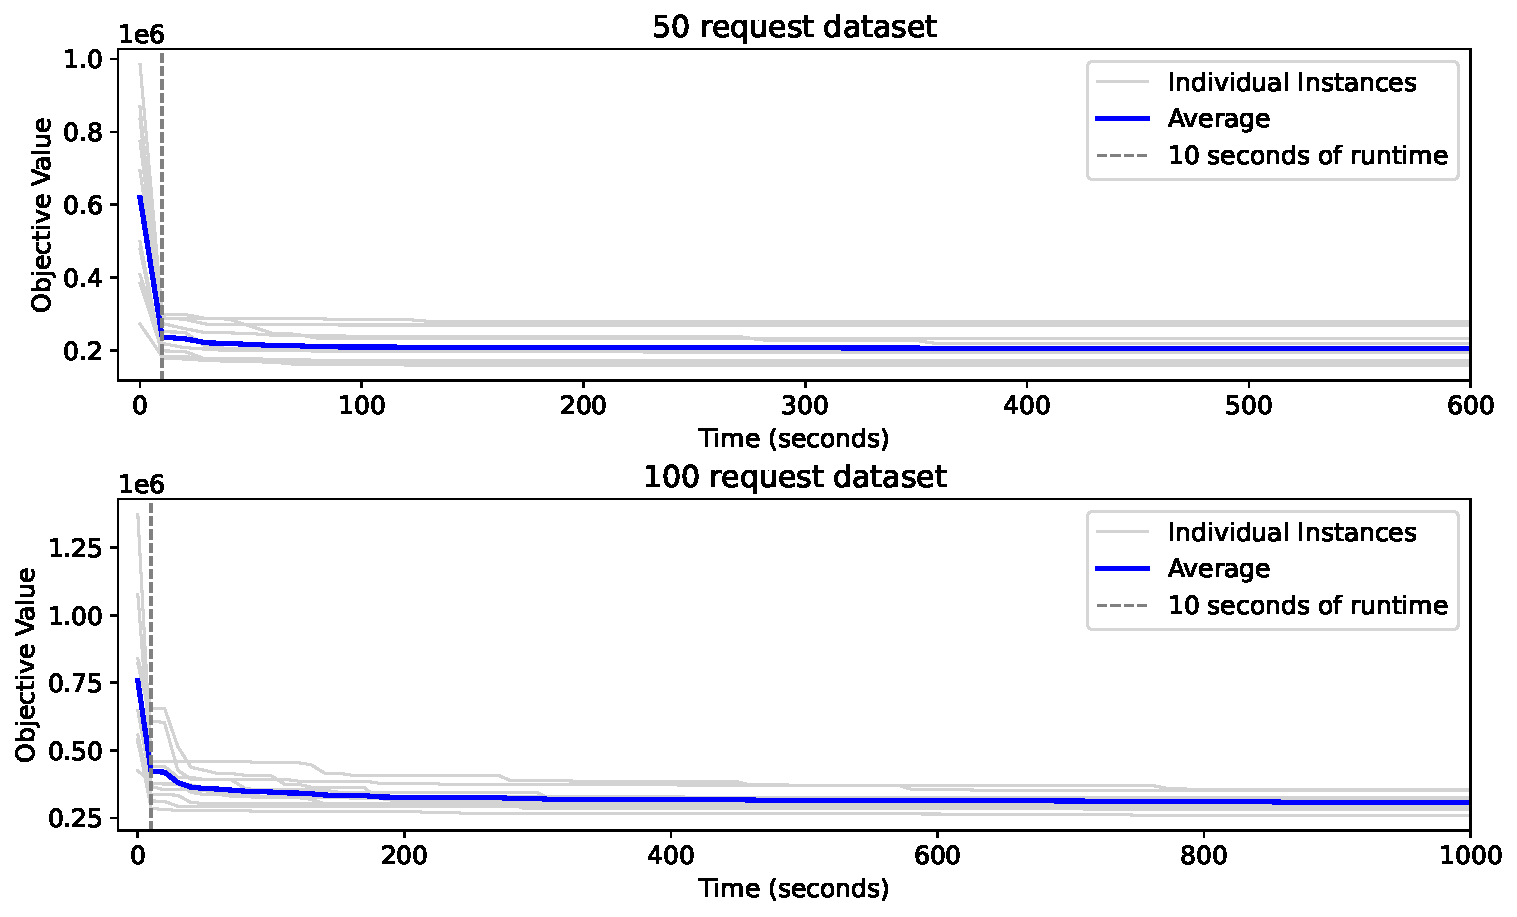
\includegraphics[width=\textwidth]{figures/graph-times.pdf}
        \caption{The evolution of the objective value through running time on 50 and 100 request datasets.}
        \label{fig:graph-times}
    \end{figure}

    \begin{figure}[!ht]
        \centering
        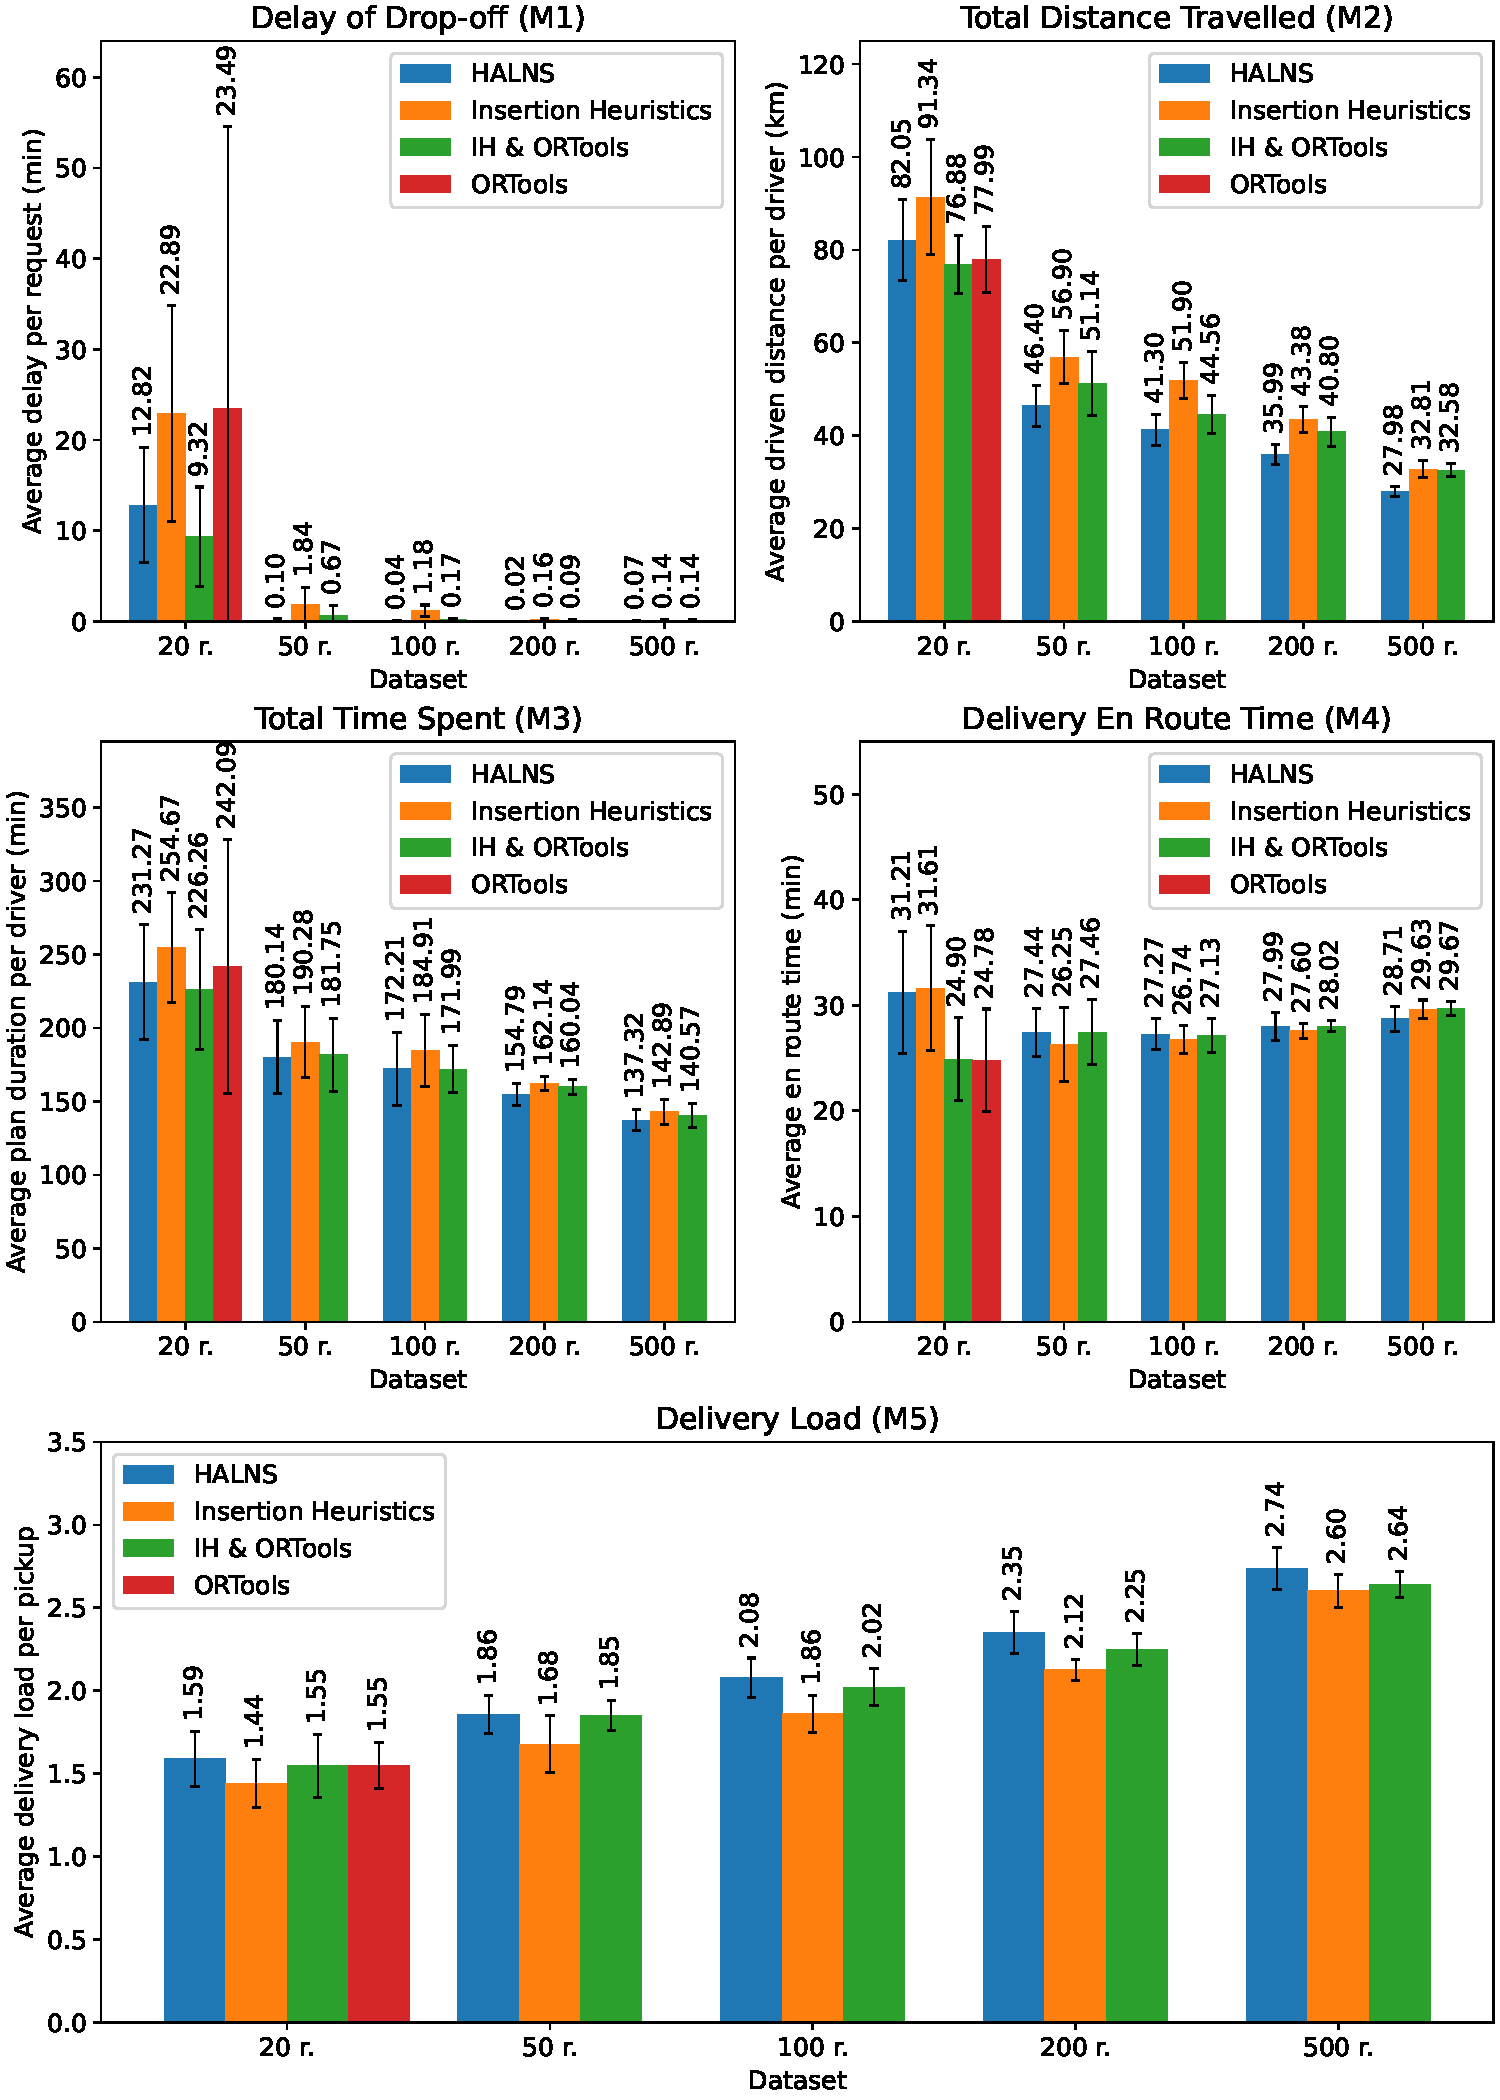
\includegraphics[width=\textwidth]{figures/metrics-graphs.pdf}
        \caption{Results of metrics M1 - M5 evaluated on our 5 datasets, averaged from 10 runs of each instance in each dataset.}
        \label{fig:metrics-graphs}
    \end{figure}
    
    
    The objective is to minimize the total delay and the total distance by using the formula $cost(e) = \beta t^{\mathrm{delay}}_e + \gamma t^{\mathrm{distance}}_e$ for each route $e$ with the parameters $\beta = 1$ and $\gamma = 0.5$, as detailed in sections \ref{halns:cost} and \ref{halns:parameters}. Therefore, we observe the tradeoff between the total delay accumulated on all requests in the instance and the total distance travelled by all drivers. The figure \ref{fig:graph-tradeoff} shows this tradeoff for each solution in our datasets. The figure \ref{fig:graph-tradeoff} confirms that the HALNS algorithm produces the overall best solutions without any outliers, compared to the baseline methods.
    
    \begin{figure}[!ht]
        \centering
        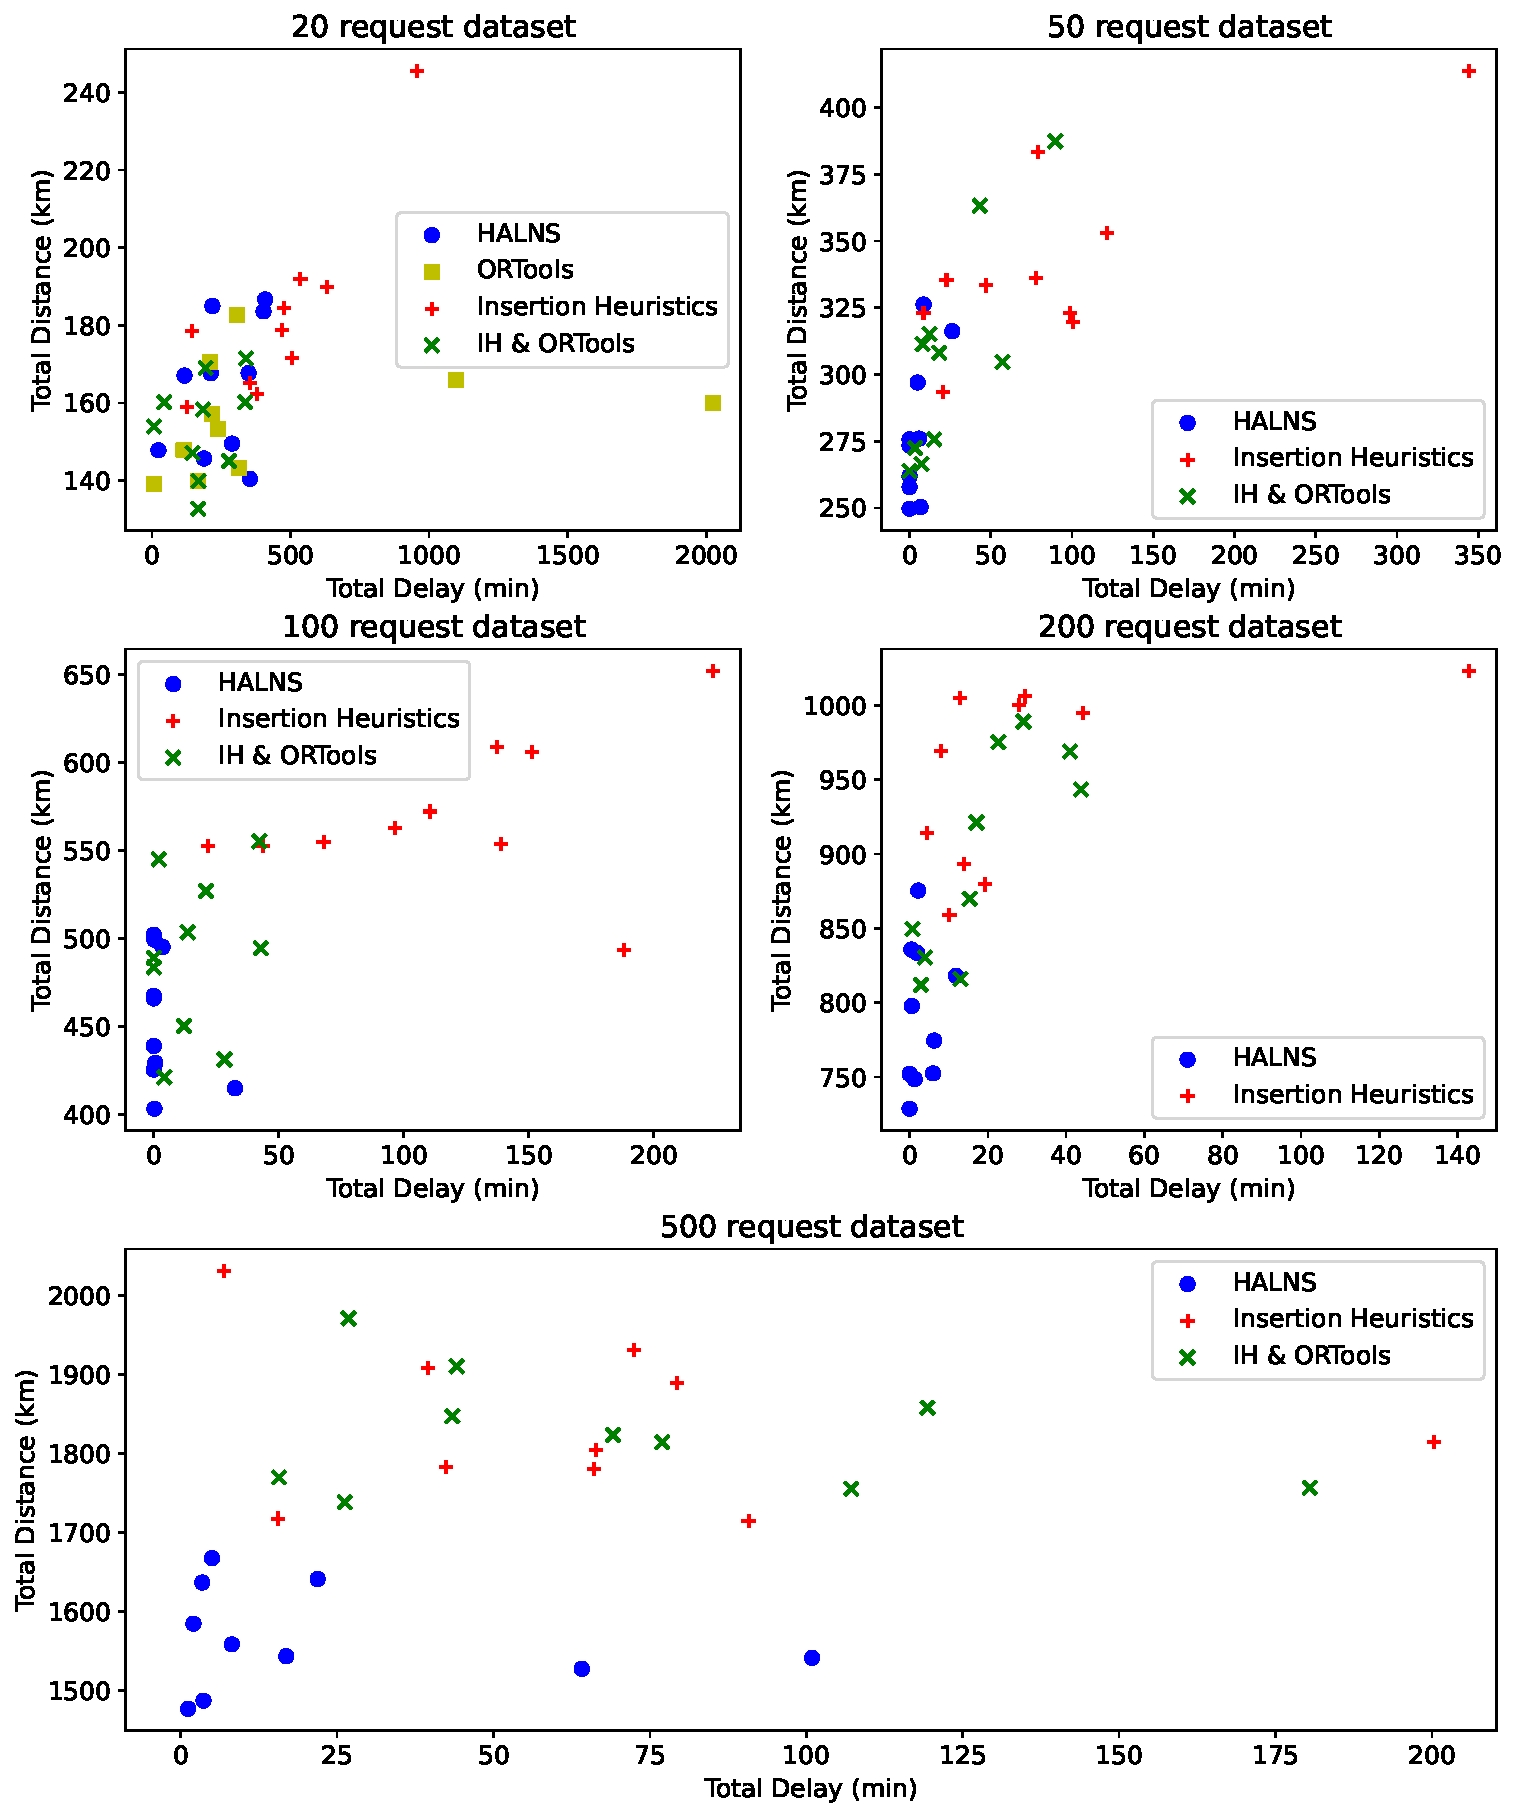
\includegraphics[width=0.9\textwidth]{figures/graph-tradeoff-2.pdf}
        \caption{The tradeoff between the total delay and the total distance for each solution produced by the individual algorithms.}
        \label{fig:graph-tradeoff}
    \end{figure}
    

    
    
    \section{Experiments on Adaptive Weight Adjustment}
    
    This section provides some results regarding the adaptive weight adjustment procedure and details the selection process of parameters $\pi_1$, $\pi_2$ and $\pi_3$ that are used to update the weights of the operators based on their past performance, as thoroughly described in section \ref{halns:weight}.
    
    To select the parameters $\pi_1$, $\pi_2$ and $\pi_3$ we conducted an experiment with different combinations of these parameters and compared the results. This experiment was run on a single dataset of 50 requests. It was executed 10 times and the results were averaged. The possible combinations are based on the study by Masmoudi et al. (2016) \cite{Masmoudi2016}. The produced solutions are in this case compared only by the objective function as only the HALNS algorithm is employed in this experiment. The results are shown in table \ref{tab:parameter-experiments}.
    
    Based on these results, the combination of parameters that works the best for this dataset is $(\pi_1, \pi_2, \pi_3) = (15, 5, 10)$, which was also used by Masmoudi et al. (2020) \cite{Masmoudi2020} and which follows the proposal of Ropke et al. (2006) \cite{Ropke2006} that $\pi_1 > \pi_3 > \pi_2$ to reinforce the diversification and thus escaping the local minima. All experiments were conducted with this set of parameters.
    
    \afterpage{
    \clearpage
    \thispagestyle{empty}
    \begin{landscape}
        \centering
        {\renewcommand{\arraystretch}{1.5}
    \begin{tabular}{llllllllll}
    \hline
    \textbf{Instance} & \multicolumn{9}{l}{\textbf{Parameters ($\pi_1$, $\pi_2$, $\pi_3$)}}                                                       		 \\ \hline
    \textbf{}         & (15, 5, 10)         &  (1, 10, 5)        &  (1, 5, 10)        &  (1, 5, 5)         &  (10, 1, 5)    &  (10, 5, 1) &  (15, 10, 5) &  (1, 1, 1) &  (5, 1, 5)        \\ \hline
    1                 & 195077   &    197960   &    195018   &   197029   &    \textbf{194462}   &    195633   &     195356   &     198399   &   195077          \\
    2                 & \textbf{214410}   &    227528   &    219882   &   219768   &    219882   &    \textbf{214410}   &     221973   &     243910   &   220435          \\
    3                 & 197892   &    196654   &    196654   &   197996   &    \textbf{196016}   &    196654   &     196075   &     197996   &   197892          \\
    4                 & \textbf{157259}   &    158263   &    \textbf{157259}   &   \textbf{157259}   &    158263   &    160289   &     158886   &     \textbf{157259}   &   \textbf{157259}          \\
    5                 & 270077   &    269402   &    274330   &   274741   &    274127   &    267039   &     \textbf{265941}   &     269740   &   269870          \\
    6                 & 164381   &    \textbf{161878}   &    163186   &   163802   &    164166   &    \textbf{161878}   &     163798   &     163798   &   163927          \\
    7                 & 278977   &    278977   &    287459   &   293440   &    280470   &    293440   &     293440   &     \textbf{277466}   &   287602          \\
    8                 & 210639   &    231503   &    213496   &   \textbf{205610}   &    235613   &    206667   &     236569   &     210842   &   214837          \\
    9                 & 172892   &    173621   &    \textbf{170469}   &   172849   &    172849   &    173098   &     173621   &     173897   &   173144          \\
    10                & 170499   &    173052   &    169367   &   \textbf{169296}   &    169870   &    171091   &     170308   &     170745   &   \textbf{169296}          \\ \hline
    \textbf{Average}  & \textbf{203210.3} &    206883.8 &    204712.0 &   205179.0 &    206571.8 &    204019.9 &     207596.7 &     206405.2 &   204933.9
    \end{tabular}}
    \captionof{table}{Quality of produced solutions on instances of 50 requests with different combinations of parameters $\pi_1$, $\pi_2$ and $\pi_3$. Values in bold represent the minima.}
    \label{tab:parameter-experiments}
    \end{landscape}
    \clearpage
    }

    
    The performance of four insertion operators and five removal operators were studied. Figures \ref{fig:graph-insertion} and \ref{fig:graph-removal} show how the weights of the operators are updated in the first 3000 iterations of the search on a single, randomly selected instance. Similarly, tables \ref{tab:res-operator-percentage-insertion} and \ref{tab:res-operator-percentage-removal} in the appendix \ref{app:tables} show the percentage of time each insertion and removal operators were used within 5 minutes of runtime on all instances of the 100 request dataset, averaged from 10 runs of each. The results in table \ref{tab:res-operator-percentage-removal} show that the removal operators have comparable frequencies of usage. The reason behind that may be the fact that in most cases two removal operators are applied. In contrast, the insertion operators are much more imbalanced. The operators I2 and I4 are used much more often than the other two, probably because these two operators are greedier in terms of finding the best insertion point across all routes rather than in a single route.
    
    \begin{figure}[!ht]
        \centering
        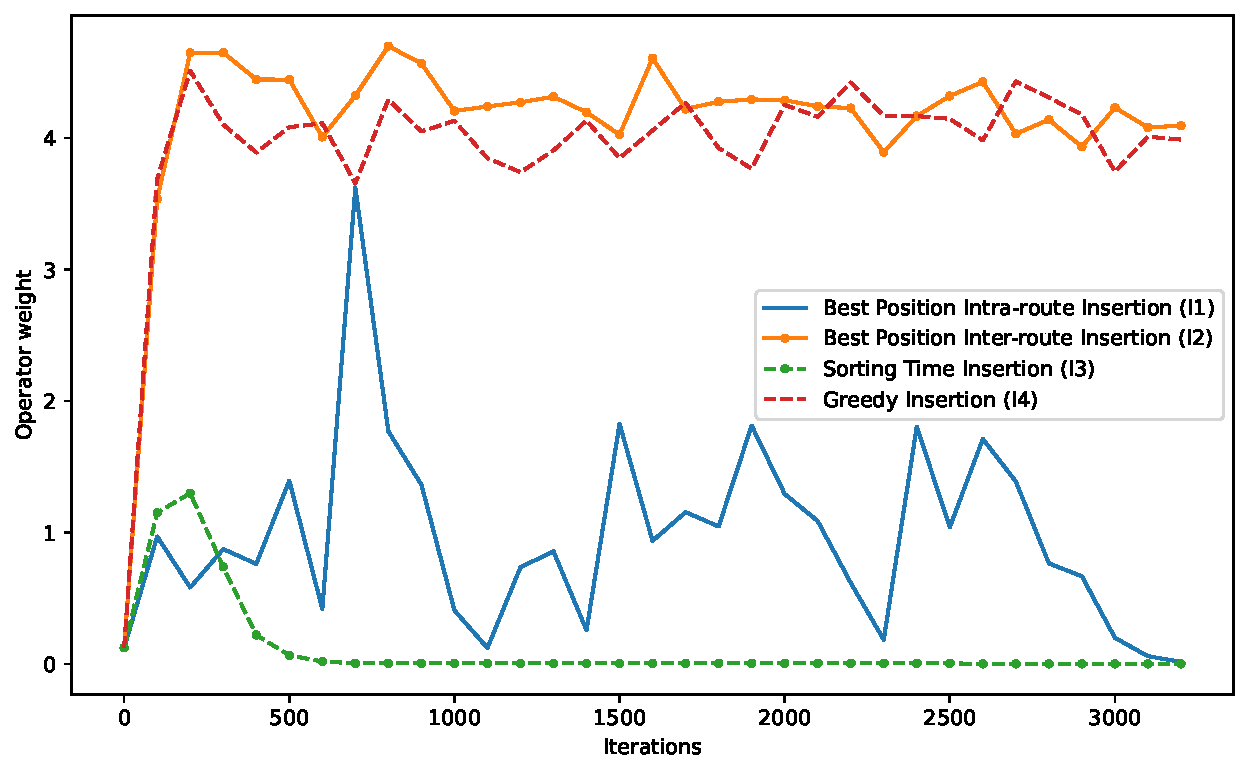
\includegraphics[width=0.9\textwidth]{figures/insertion-operators.pdf}
        \caption{Update of the weights of our four insertion operators during the first 3\,000 iterations on a single instance.}
        \label{fig:graph-insertion}
    \end{figure}
    
    \begin{figure}[!ht]
        \centering
        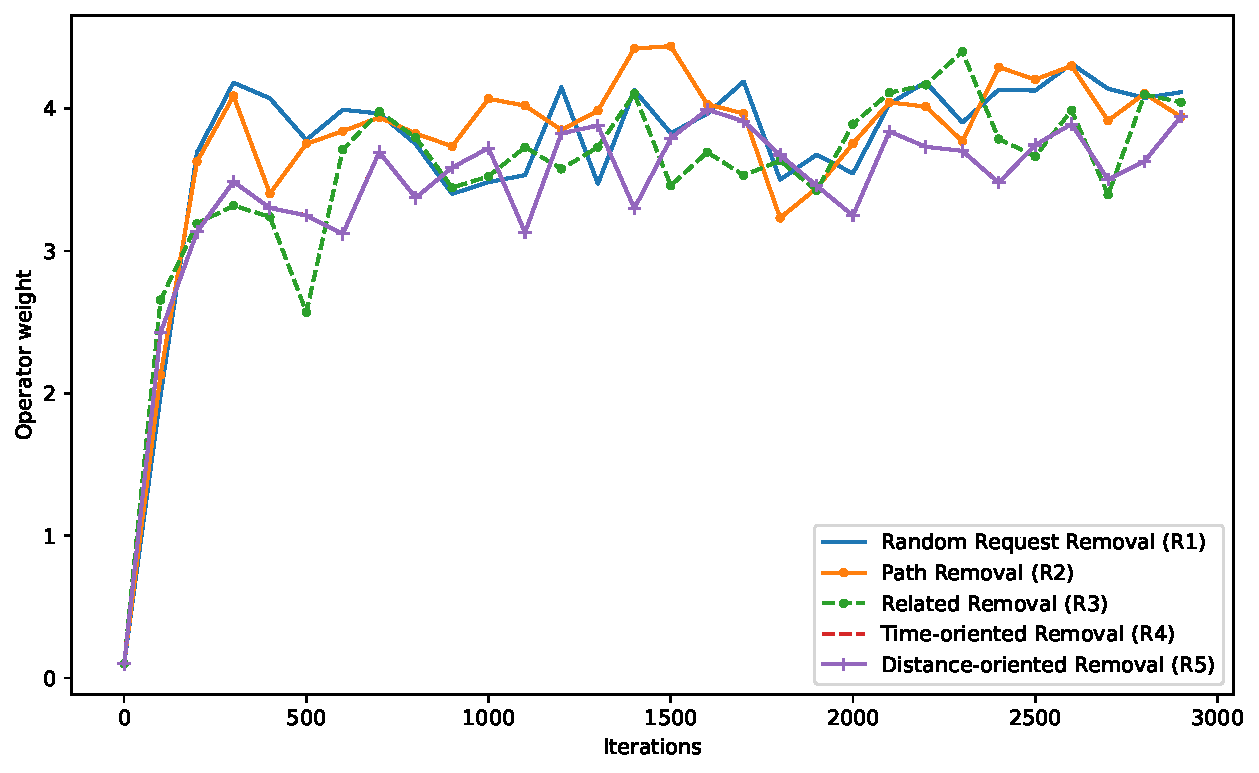
\includegraphics[width=0.9\textwidth]{figures/removal-operators.pdf}
        \caption{Update of the weights of our five removal operators during the first 3\,000 iterations on a single instance.}
        \label{fig:graph-removal}
    \end{figure}

    
    
    We also studied the complexity of the insertion and removal operators using the Go profiler. Table \ref{tab:operators-cpu} shows the CPU time used by each operator within 5 minutes of runtime. As expected, the greedy insertion operator I4 takes the most CPU time.
